\section{模型评价和改进}

\subsection{模型优点}

\begin{enumerate}
  \item 本文使用特征编码将数据集中的类别特征巧妙转化为数值特征,便于分析特征,以便提高模型的精度。
  \item 本文充分考虑到变量与变量之间的相关性,使用主成分分析法对原有的数据进行降维,可以使得特征的选择更加客观。
  \item 在问题三中通过施加噪音对模型的灵敏度进行分析,可以使得模型评价更为客观。
  \item 对于回归任务利用线性加权的得到更加精确的回归模型,极大的提高了模型的精度和科学性。
  \item 对于问题四不仅找到与术后满意度关联的因素,还进一步利用随机森林挖掘出了关联因素的分类规则。
\end{enumerate}




\subsection{基于Voting的模型推广}

对于问题一中的分类任务,本文考虑模型的数学可解释性,同时鉴于经过上采样和适当的数据预处理、特征工程处理后的二分类问题应当有优异的性能,未使用一些复杂的机器学习算法,取而代之的是兼具较好性能和数学可解释性的K最近邻算法。然而题设背景为临床医学,这无疑要求本文提供一个尽可能最优的不良反应预判模型——尽管这个模型数学可解释性可能不强。

对于分类任务来说,学习器从类别标记集合中预测出一个标记,最常见的组合策略是使用投票法,记学习器${{h}_{i}}$在样本$\overrightarrow{x}$上预测输出为一个$N$维向量:

\begin{equation}
    \left( h_{i}^{1}\left( \overrightarrow{x} \right),h_{i}^{2}\left( \overrightarrow{x} \right),\cdots ,h_{i}^{N}\left( \overrightarrow{x} \right) \right).
\end{equation}
其中$h_{i}^{j}\left( \overrightarrow{x} \right)$是${{h}_{i}}$在类别标记上的输出。

\begin{figure}[H] % 这个H不要动!
	\centering % 不要动!
	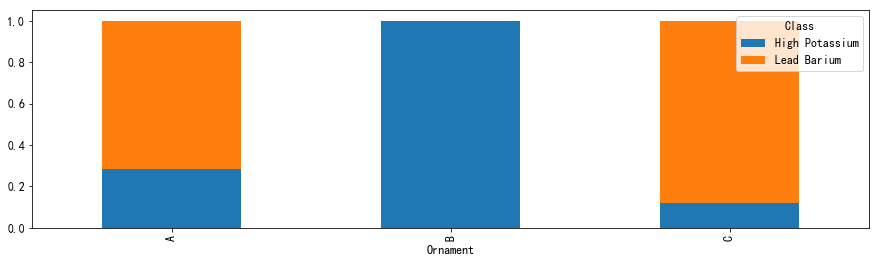
\includegraphics[width=0.95\textwidth]{14.png} 
	\caption{Voting原理图} 
	\label{Fig.main14} 
\end{figure}


对于分类模型,本文欲基于模型融合算法VotingClassifier将多个性能优良的基分类器融合在一起。下文中的分析与评价均以“呛咳”为标签的分类任务为例。本文选取7个经典的分类模型,经过训练集训练后在测试集上测试,以Accuracy\_score为初步的评价指标,结果如下:

\begin{table}[H]
    \centering  
    \caption{分类器泛化能力评价——以Accuracy\_score为指标}
    \begin{tabular}{c c c}  
    	\toprule[1.5pt]  
    	分类器        & Accuracy\_score \\  
    	\midrule[1pt]    
    	逻辑回归      & 0.646 \\ 
    	线性判别分析  & 0.63941 \\ 
    	K最近邻       &  0.90985 \\ 
    	决策树        & 0.97694 \\ 
    	朴素贝叶斯    &  0.61635 \\ 
    	支持向量机    & 0.66247 \\ 
    	XGBoost       &  0.97904 \\ 
    	\toprule[1.5pt]  
    \end{tabular}  
\end{table} 

基于上面的初步测试,本文选择决策树、K最近邻、XGBoost、Catboost作为基分类器,通过Voting中的软投票对四个分类器进行融合,结果如下:

\begin{table}[H]
    \centering  
    \caption{Voting与基分类器性能对比}
    \begin{tabular}{c c c}  
    	\toprule[1.5pt]  
    	分类器        & Accuracy\_score \\  
    	\midrule[1pt]    
    	XGB & 0.97904 \\
        KNN & 0.90985 \\
        DT  & 0.97694 \\
        Voting & 0.98113 \\
    	\toprule[1.5pt]  
    \end{tabular}  
\end{table} 

进一步地,为了更直观地展示Voting的泛化能力,本文通过混淆矩阵和ROC图对Voting的性能进行可视化:

\begin{figure}[H] % 这个H不要动!
	\centering % 不要动!
	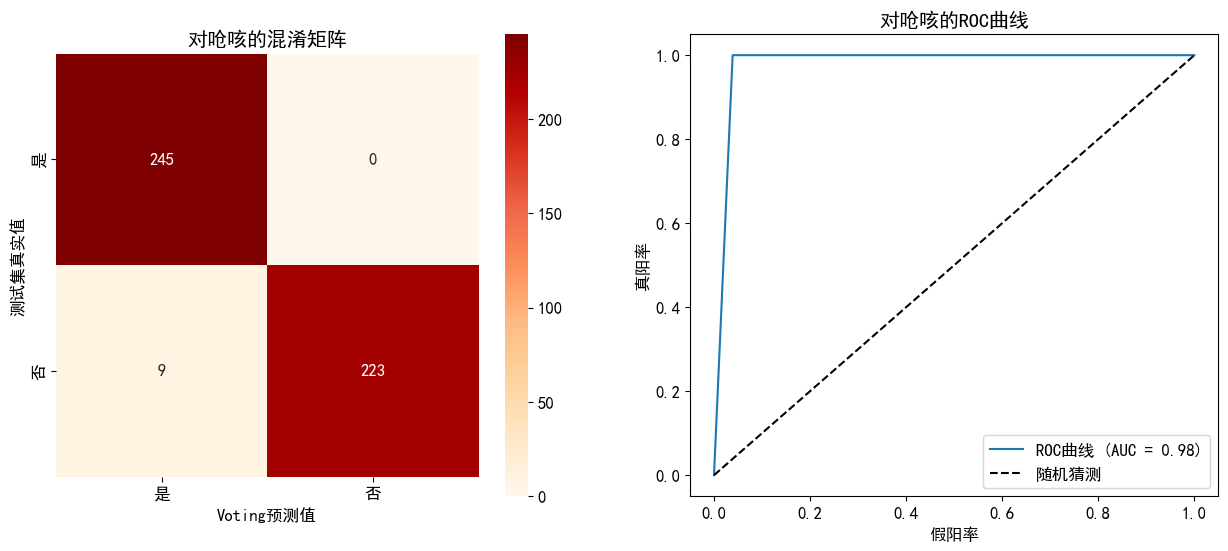
\includegraphics[width=0.95\textwidth]{13.png} 
	\caption{Voting的混淆矩阵与ROC图} 
	\label{Fig.main13} 
\end{figure}

可以见得Voting的分类性能要比KNN更好,将其应用在临床医学中才更符合人工智能服务人类的初衷。












